% Specifica che tipo di documento vuoi creare
\documentclass[presentation]{beamer}\mode<presentation>{
% Specifica il tema da usare
\usetheme{Warsaw}}
\usecolortheme{seahorse}
% Si possono dichiarare dei pacchetti che contengono comandi aggiuntivi
\usepackage[english]{babel} % Supporta caratteri inglesi
\usepackage[italian]{babel} % Supporta caratteri accentati italiani
\usepackage[utf8]{inputenc}

% Altri comandi aggiuntivi
\usepackage{verbatim}
%\usepackage{soul}
\usepackage{amsmath}
\usepackage{amssymb}
\usepackage{textcomp}

\institute
{Politecnico di Torino \par 
Corso di Laurea Magistrale in Ingegneria Biomedica}

\title
{Costruzione di un classificatore basato su Logica Fuzzy}

\subject{Classificazione ed Interpretazione dei Dati Biomedici}

\author\right
{Arianna Roma \par Matricola: 208816 }

%
% Cambiate la data se volete, diversamente LaTeX mette la data odierna
\date{11 febbraio 2015}

%% Da qui specificate cosa deve apparire
%\begin{document}
%
%% Crea una slide per il titolo
%\frame[label=coverpage]{\titlepage}
%
%%Crea una slide per l'indice in modo automatico, se usate section e subsection
%\frame{\tableofcontents}
%
%\section{Questa è una sezione}
%\subsection{che contiene una sottosezione}
%% Slides fatte a mano
%\begin{frame}{Questo è un titolo}
%Qui inserisco una figura
%\begin{figure}[H]
%  \begin{center} %La voglio centrata
%    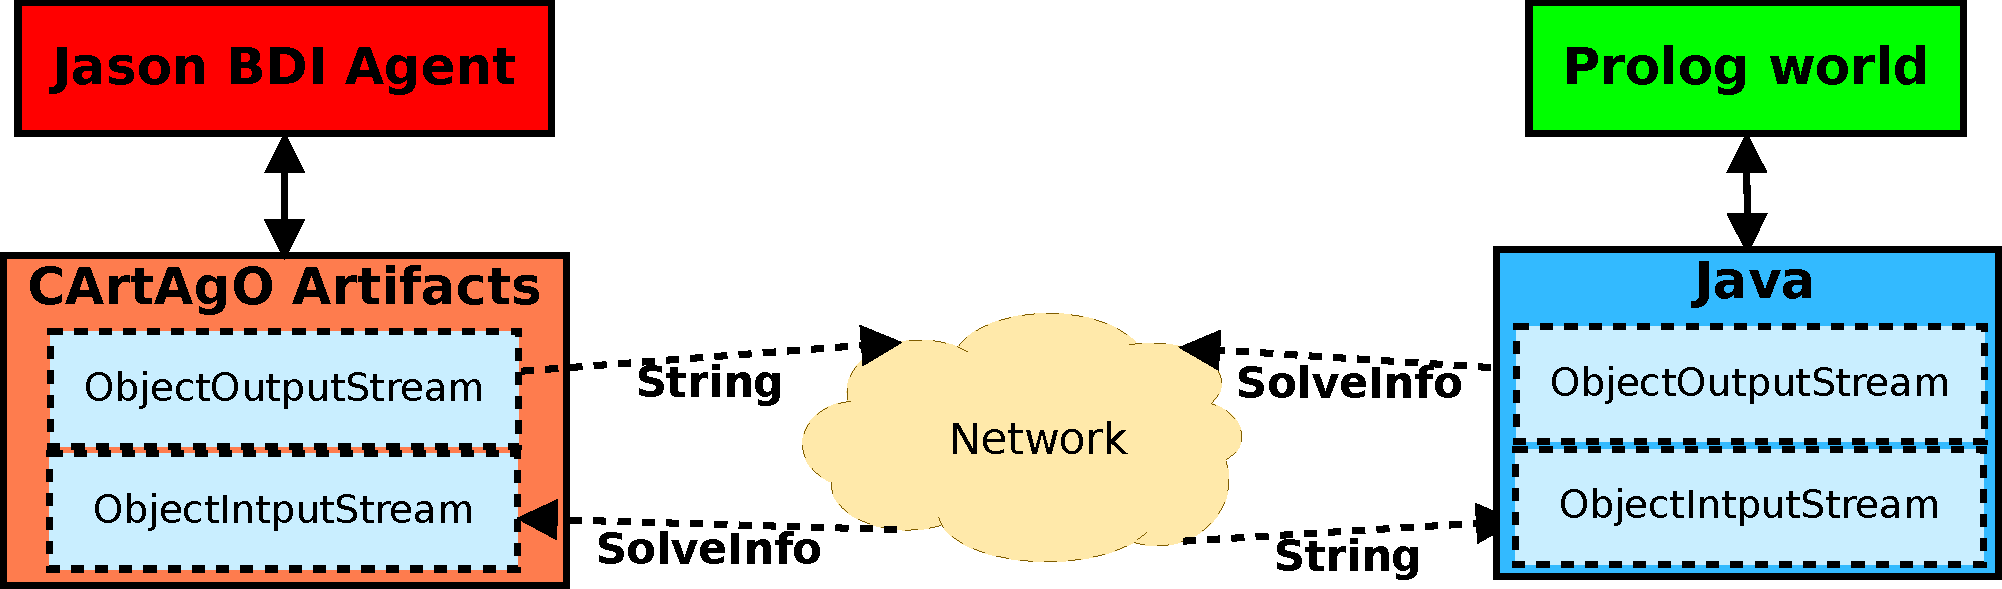
\includegraphics[width=0.99\textwidth]{img/graph.pdf}
%  \end{center}
%  \caption{Una didascalia}
%  \label{riferimentoFigura}
%\end{figure}
%\end{frame}
%
%\begin{frame}{Un'altra slide}
%Creiamo un box\\vado\\a\\capo
%
%Anche così vado a capo.
%Così no.
%\end{frame}
%
%\subsection{e un'altra sottosezone}
%\begin{frame}{\LaTeX\ è fatto per la matematica}
%ciao
%Equazione da mettere $\frac{1}{\sqrt{2\pi}}\int_{-\infty}^{\infty}f(t)\cdotp e^{j\omega t} dt $ in mezzo al testo 
%
%Equazione da mettere $$\frac{1}{\sqrt{2\pi}}\int_{-\infty}^{\infty}f(t)\cdotp e^{j\omega t} dt $$ a parte
%
%Equazione SERIA
%\begin{equation}
%\frac{1}{\sqrt{2\pi}}\int_{-\infty}^{\infty}f(t)\cdotp e^{j\omega t} dt
%\label{fourier}
%\end{equation}
%le equazioni serie possono essere referenziate, vedi Equazione \ref{fourier}
%\end{frame}
%
%\begin{frame}{\LaTeX\ si sbatte per capire dove hai messo la roba}
%\label{slideref} % etichetta per il frame
%Se avete usato \texttt{$\backslash$label} correttamente, potete anche fare riferimento alle sezioni, ad esempio alla Sezione \ref{sec:riferimento} o alla Sottosezione \ref{subsec:riferimento}, oppure ai frames. Ad esempio, per riferire me stesso posso citare la Slide \ref{slideref}
%\end{frame}
%
%\subsection*{oltre ad una sezione che non voglio vedere nell'indice}
%\begin{frame}{\LaTeX\ supporta gli elenchi}
%\begin{itemize}
% \item Questo
% \item elenco
% \item non
% \item è
% \item numerato
%\end{itemize}
%\begin{enumerate}
% \item Questo
% \item elenco
% \item è
% \item numerato
%\end{enumerate}
%\end{frame}
%
%\subsection{Mettendo * dopo section e subsection, l'indice le ignora!}
%\label{subsec:riferimento}
%\begin{frame}{Tipografia}
%Si può scrivere in \textbf{grassetto}, \textsc{maiuscoletto}, in \textit{corsivo}, \emph{enfatizzato} (ovvero sceglie \LaTeX in base al testo che lo circonda), \underline{sottolineato}, \texttt{equispaziato} (ottimo per il codice, ad esempio \texttt{public static void main(String[] a)})
%\end{frame}
%
%\section{Sezione 2 senza sottosezioni, con riferimento}
%\label{sec:riferimento}
%\begin{frame}[fragile]{Potete scriverci del codice}
%\begin{verbatim}
%clear
%clc
%[STARTTIME1,FREQUENCY1,EMGMAP1,LABELS1,EMGDATA1] = TDFREADDATAEMG ('max_TA_1.tdf');
%[STARTTIME,FREQUENCY,EMGMAP,LABELS,EMGDATA] = TDFREADDATAEMG ('max_GC_1.tdf');
%TA=EMGDATA1(1,:);
%GC_filtrato=filtfilt(num,den,GC_abs);
%figure(3);
%plot(TA_filtrato)
%figure(4);
%plot(GC_filtrato)
%for i=1:151
%    EMG_GC_filtrato(1,i)=mean(GC_filtrato(:,(100*(i-1)+1):(100*i)));
%end
%\end{verbatim}
%\end{frame}
%
%\section{Sezione 3}
%\subsection{Pippo}
%\begin{frame}{Dimensionate il testo}
%\tiny
%tiny
%
%\scriptsize
%scriptsize
%
%\footnotesize
%footnotesize
%
%\small
%small
%
%\normalsize
%normalsize (default)
%
%\large
%large
%
%\Large
%Large (capital "L")
%
%\LARGE
%LARGE (all caps)
%
%\huge
%huge
%
%\Huge
%Huge (capital "H")
%\end{frame}
%
%\begin{frame}{I box sono fighi!!}
%Si possono fare dei box!
%\begin{block}{Titolo del box}
%Contenuto del box 
%\end{block}
%\begin{block}{Ovviamente}
%Il contenuto può essere qualunque cosa
%\begin{itemize}
% \item anche
% \item un
% \item elenco
%\end{itemize}
%\begin{enumerate}
% \item o 
% \item una
% \item enumerazione
%\end{enumerate}
%\end{block}
%\end{frame}
%
%\subsection{Pluto}
%\begin{frame}{Teoremi}
%\begin{theorem}
%Teorema di Pianini:\\
%L'integrale lungo il cavallo chiuso
%\begin{equation}
%\biguplus \bigotimes \intercal \boxtimes \odot \star \ast \div \divideontimes \ltimes \textcurrency
%\label{eq:theorem}
%\end{equation}
%Vale la roba che c'è sopra
%\label{teorema}
%\end{theorem}
%Ovviamente ci si può riferire a quel cazzo di Teorema \ref{teorema}, ma anche all'Equazione \ref{eq:theorem} che ci sta dentro.
%\end{frame}
%
%
%
%
%%===============================================================================
%\againframe{coverpage}
%%===============================================================================
%%%%%%%%%%%%%%%%%%%%%%%%%%%%%%%%%%%%%%%%%%%%%%%%%%%%%%%%%%%%%%%%%%%%%%%%%%%%%%%%%
%\end{document}
%%%%%%%%%%%%%%%%%%%%%%%%%%%%%%%%%%%%%%%%%%%%%%%%%%%%%%%%%%%%%%%%%%%%%%%%%%%%%%%%%